%% For double-blind review submission, w/o CCS and ACM Reference (max submission space)
\documentclass[sigplan,10pt,screen]{acmart}
\settopmatter{printfolios=true,printccs=false,printacmref=false}
\renewcommand\footnotetextcopyrightpermission[1]{} % removes footnote with conference information in first column

\acmConference[POPL SRC 2018]{}{January 11, 2018}{Los Angeles, CA, USA}
\setcopyright{none}

%% Bibliography style
\bibliographystyle{acm-reference-format}
%% Citation style
\citestyle{acmnumeric}     %% For numeric citations


%%%%%%%%%%%%%%%%%%%%%%%%%%%%%%%%%%%%%%%%%%%%%%%%%%%%%%%%%%%%%%%%%%%%%%
%% Note: Authors migrating a paper from traditional SIGPLAN
%% proceedings format to PACMPL format must update the
%% '\documentclass' and topmatter commands above; see
%% 'acmart-pacmpl-template.tex'.
%%%%%%%%%%%%%%%%%%%%%%%%%%%%%%%%%%%%%%%%%%%%%%%%%%%%%%%%%%%%%%%%%%%%%%


%% Some recommended packages.
\usepackage{booktabs}   %% For formal tables:
                        %% http://ctan.org/pkg/booktabs
\usepackage{subcaption} %% For complex figures with subfigures/subcaptions
                        %% http://ctan.org/pkg/subcaption

\usepackage[T1]{fontenc}
\usepackage[utf8]{inputenc}
\usepackage{listings}
\usepackage{todonotes}
\usepackage{graphviz}

\newcommand{\ottifc}{Ott-IFC}
\newcommand{\config}[3]{\ensuremath{\langle #1, #2, #3 \rangle}}
\newcommand{\emits}[3]{\ensuremath{#2\downarrow_{#1}#3}}
\newcommand{\proj}[2]{\ensuremath{{#1 \! \upharpoonright  \! {#2}}}}
\newcommand{\step}{{\ensuremath{\Downarrow}}}

\definecolor{grey}{rgb}{0.8,0.8,0.8}
\definecolor{code-background}{RGB}{255, 248, 220}
\definecolor{code-comment}{RGB}{196, 42, 42}
\definecolor{code-linenumber}{rgb}{0.5,0.5,0.5}
\definecolor{code-keyword}{RGB}{148, 0, 211}
\definecolor{coqatoo-pink}      {RGB}{255, 107, 104}
\definecolor{coqatoo-gray}      {RGB}{64, 64, 64}
\definecolor{coqatoo-yellow}    {RGB}{239, 223, 0}
\lstset{
   backgroundcolor=\color{code-background},   	% choose the background color; you must add \usepackage{color} or \usepackage{xcolor}
   basicstyle=\tt\footnotesize,       			% the size of the fonts that are used for the code
   breakatwhitespace=false,         			% sets if automatic breaks should only happen at whitespace
   breaklines=true,                 			% sets automatic line breaking
   captionpos=none,                    			% sets the caption-position to bottom
   commentstyle=\color{code-comment},   		% comment style
   deletekeywords={...},            			% if you want to delete keywords from the given language
   escapeinside={\%*}{*)},          			% if you want to add LaTeX within your code
   extendedchars=true,              			% lets you use non-ASCII characters; for 8-bits encodings only, does not work with UTF-8
   frame=tb,
   framerule=0pt,
   framextopmargin=0pt,
   framexbottommargin=0pt,
   keepspaces=true,                 			% keeps spaces in text, useful for keeping indentation of code (possibly needs columns=flexible)
   keywordstyle=\color{code-keyword},       						% keyword style
   language=ML,                 				% the language of the code
   morekeywords={Lemma, Proof, Qed, if, then, else, end, skip, stop, read, from, write, to},            % if you want to add more keywords to the set
   numbers=none,                    			% where to put the line-numbers; possible values are (none, left, right)
   numbersep=5pt,	                   			% how far the line-numbers are from the code
   numberstyle=\tiny\color{code-linenumber}, 	% the style that is used for the line-numbers
   rulecolor=\color{black}, 	        		% if not set, the frame-color may be changed on line-breaks within not-black text (e.g. comments (green here))
   showspaces=false,            	    		% show spaces everywhere adding particular underscores; it overrides 'showstringspaces'
   showstringspaces=false,          			% underline spaces within strings only
   showtabs=false,                  			% show tabs within strings adding particular underscores
   stepnumber=1,                    			% the step between two line-numbers. If it's 1, each line will be numbered
   stringstyle=\color{black},            		% string literal style
   tabsize=2,                       			% sets default tabsize to 2 spaces
   gobble=0,									% number of characters to remove at the beginning of each line
   mathescape=true,								% to render math symbols in the listing (between $)
   title=\lstname,                   			% show the filename of files included with \lstinputlisting; also try caption instead of title
   belowcaptionskip = 0cm
}

\begin{document}

%% Title information
\title[ott-ifc]{Ott-IFC: Generating Information-Flow Control Mechanisms}


%% Author information
\author{Andrew Bedford}
\orcid{0000-0003-3101-4272}             %% \orcid is optional
\affiliation{
  \institution{Laval University}            %% \institution is required
  \state{Quebec}
  \country{Canada}                    %% \country is recommended
}
\email{andrew.bedford.1@ulaval.ca}          %% \email is recommended


% Abstract
\begin{abstract}
Developing information-flow control mechanisms can be a difficult and time-consuming task, particularly when dealing with complex programming languages. 

To help with this task, we have developed a tool called \emph{\ottifc} that can automatically generate information-flow control mechanisms from programming language specifications (i.e., syntax and semantics).
\end{abstract}

\maketitle

\section{Introduction}
Modern operating systems rely mostly on access-control mechanisms to protect users information. However, access control mechanisms are insufficient as they cannot regulate the propagation of information once it has been released for processing. To address this issue, a new research trend called \emph{language-based information-flow security}~\cite{DBLP:journals/jsac/SabelfeldM03} has emerged. The idea is to use techniques from programming languages, such as program analysis, monitoring, rewriting and type checking, to enforce information-flow policies (e.g., information from a private file should not saved in a public file). Mechanisms that enforce such policies (e.g., \cite{DBLP:journals/jcs/VolpanoIS96, DBLP:conf/csfw/ChudnovN10,DBLP:journals/compsec/BedfordCDKT17}) are called \emph{information-flow control mechanisms}. 

Information-flow control mechanisms are usually designed and implemented completely by a human. Developing sound mechanisms can be a challenging task, particularly when dealing with complex programming languages, due to the numerous ways through which information may flow in a program. In order to make this process less laborious and reduce the risk of errors, we have created a tool called \ottifc\ that takes as input a programming language's specification (i.e., syntax and semantics) and produces a mechanism's specification (e.g., runtime monitor).

\paragraph{Contributions}
\begin{itemize}
	\item We present \ottifc\ in Section~\ref{section:ott-ifc}.
	\item We prove that the mechanisms generated by \ottifc\ are sound in Section~\ref{section:soundness}.
	\item We discuss \ottifc's limitations in Section
\end{itemize}

%Background and Related Work: Describe the specialized (but pertinent) background necessary to appreciate the work. Include references to the literature where appropriate, and briefly explain where your work departs from that done by others.
\newpage
\section{Background}\label{section:background}
Most information-flow control mechanisms seek to enforce a policy called \emph{non-interference}~\cite{DBLP:conf/sp/GoguenM82a}, which essentially states that private information may not interfere with the publicly observable behavior of a program. To enforce non-interference, a mechanism must take into account two types of information flows: \emph{explicit flows} and \emph{implicit flows}~\cite{DBLP:journals/cacm/Denning76}. 

An insecure explicit information flow (Listing~\ref{listing:explicit-flow}) occurs when private information flows directly into public information. 
\begin{lstlisting}[captionpos=b, caption=Insecure explicit flow, label=listing:explicit-flow]
  public := private
\end{lstlisting}
Explicit flows can be prevented by associating labels to sensitive information and propagating them whenever the information is used; a process known as \emph{tainting}.

An insecure implicit information flow (Listing~\ref{listing:implicit-flow}) occurs when private information influences public information\\through the control-flow of the application.

\begin{lstlisting}[captionpos=b, caption=Insecure implicit flow, label=listing:implicit-flow]
  if (private > 0) then
    public := 0
  else
    public := 1
  end
\end{lstlisting}
Implicit flows can be prevented using a program counter, $pc$, which keeps track of the context in which a command is executed.

%Approach and Uniqueness: Describe your approach in attacking the problem and clearly state how your approach is novel.
\section{Ott-IFC}\label{section:ott-ifc}
As the name implies, the specifications that \ottifc\ takes as input (and outputs) are written in Ott~\cite{DBLP:journals/jfp/SewellNOPRSS10}. Ott is a tool that can generate LaTeX, Coq or Isabelle/HOL versions of a programming language's specification. The specification is written in a concise and readable ASCII notation that ressembles what one would write in informal mathematics (see following Listings).

Hence, the development process of a mechanism using Ott and \ottifc\ would look like this:
\begin{enumerate}
  \item Write a specification of the language on which we want to enforce non-interference in Ott.
  \item Use \ottifc\ to generate the mechanism.
  \item Use Ott to export the mechanism to LaTeX/Coq/Isabelle/HOL and complete the implementation.
\end{enumerate}

\todo[inline]{pseudocode}
\todo[inline]{identifying commands and expressions}
\todo[inline]{unfolding productions}

For the moment, \ottifc\ supports only languages whose specification respects certain rules. Namely, that the syntax be composed of expressions, which may only read the memory, and commands, which may read or write the memory; and that the program configurations be of the form $\langle command, memory\rangle$. 

To illustrate our approach, consider the imperative language whose syntax is defined in Listing~\ref{listing:input-syntax} and (partial) semantics in Listings~\ref{listing:input-semantics-assign} and \ref{listing:input-semantics-if}.

\begin{lstlisting}[label=listing:input-syntax,captionpos=b,caption=Ott syntax of a simple imperative language]
  arith_expr, a ::= x | n | a1 + a2 | a1 * a2 
  bool_expr, b ::= true | false | a1 < a2
  commands, c ::= skip | x := a | c1 ; c2 | 
                  read x from ch | write x to ch |
                  if b then c1 else c2 end | 
                  while b do c end

\end{lstlisting}

%\begin{lstlisting}[label=listing:input-semantics-assign,captionpos=b,caption={Ott big-step semantics of the assign command}]
%  <a, m, o> || <n, m, o>
%  ---------------------------------
%  <x := a, m, o> || <stop, m[x |-> n], o>
%\end{lstlisting}

\begin{figure*}[h]
\begin{minipage}[t]{0.49\linewidth}
\begin{lstlisting}
$$
<a, m, o> || <n, m, o>
-----------------------------------------------------
<x := a, m, o> || <stop, m[x |-> n], o>
$$
\end{lstlisting}        
\end{minipage}
\hfill%
\begin{minipage}[t]{0.49\linewidth}
\begin{lstlisting}
<a, m, o, pc, E> || <n, m, o, pc, E>
E |- a : la
-----------------------------------------------------
<x := a, m, o, pc, E> || <stop, m[x |-> n], o, pc, 
E[x |-> pc |_| la]>
\end{lstlisting}
\end{minipage}
\end{figure*}

\begin{figure*}
\begin{minipage}[t]{0.49\linewidth}
		\begin{lstlisting}
		$$
		$$
		$$
		m(x) = n
		-----------------------------------------------------
		<write x to ch, m, o> || <stop, m[ch |-> n], 
		o::(ch ; n)>
		\end{lstlisting}        
\end{minipage}
\hfill%
\begin{minipage}[t]{0.49\linewidth}
		\begin{lstlisting}
		E |- x : lx
		E |- ch : lch
		lx |_| pc <= lch
		m(x) = n
		-----------------------------------------------------
		<write x to ch, m, o, pc, E> ||  <stop, m[ch |-> n], 
		o::(ch ; n), pc, E>
		\end{lstlisting}
\end{minipage}
\end{figure*}
\begin{figure*}
\begin{minipage}[t]{0.49\linewidth}
		\begin{lstlisting}
		$$
		$$
		<b, m, o> || <true, m, o>
		<c1, m, o> || <stop, m1, o1>
		-----------------------------------------------------
		<if b then c1 else c2 end, m, o> || <stop, m1, o1>
		
		
		
		
		<b, m, o> || <false, m, o>
		<c2, m, o> || <stop, m2, o2>
		-----------------------------------------------------
		<if b then c1 else c2 end, m, o> || <stop, m2, o2>
		$$
		\end{lstlisting}        
\end{minipage}
\hfill%
\begin{minipage}[t]{0.49\linewidth}
		\begin{lstlisting}
		E |- b : lb
		<b, m, o, pc, E> || <true, m, o, pc, E>
		<c1, m, o, pc |_| lb, E> || <stop, m1, o1, pc |_| lb, E>
		E1 = updateModifVars(E, pc, b, c2)
		-----------------------------------------------------
		<if b then c1 else c2 end, m, o, pc, E> ||  <stop, m1, o1, pc, E1>
		
		E |- b : lb
		<b, m, o, pc, E> || <false, m, o, pc, E>
		<c2, m, o, pc |_| lb, E> || <stop, m2, o2, pc |_| lb, E>
		E2 = updateModifVars(E, pc, b, c1)
		-----------------------------------------------------
		<if b then c1 else c2 end, m, o, pc, E> ||  <stop, m2, o2, pc, E2>
		\end{lstlisting}
\end{minipage}
\end{figure*}

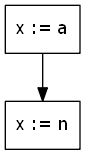
\includegraphics[width=0.25\linewidth]{images/graph-assign.png}

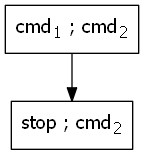
\includegraphics[width=0.25\linewidth]{images/graph-sequence.png}

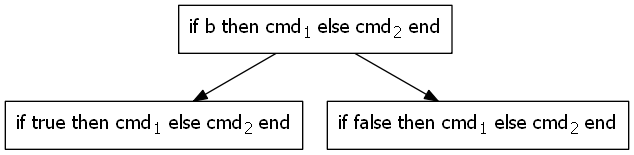
\includegraphics[width=\linewidth]{images/graph-if.png}

In order to automatically apply the techniques described in Section~\ref{section:background}, \ottifc\ starts by inserting a typing environment \lstinline{E} (which maps variables to their label) and a program counter \lstinline{pc} in each semantic rules. That is, the configurations \lstinline{<c, m>} are changed to \lstinline{<c, m, E, pc>}.

To prevent explicit flows, it identifies the semantic rules that may modify the memory \lstinline{m} (e.g., Listing~\ref{listing:input-semantics-assign}). In each of those rules, it inserts a condition to ensure that private information is not stored into a public variable and updates the modified variable's (\lstinline{x} here) label with the label of the expressions that are used in the rule.

%\begin{lstlisting}[label=listing:input-semantics-assign,captionpos=b,caption={Ott big-step semantics of the assign command}]
%  <a, m> || <n, m>
%  E |- a : ta
%  E |- x : tx
%  ta <= tx
%  ---------------------------------
%  <x:=a, m, E, pc> || <skip, m[x |-> n], E[x |-> ta], pc>
%\end{lstlisting}

To prevent implicit flows, it identifies commands that may influence the control-flow of the application. That is, commands for which a program configuration may lead to two different program configurations (e.g., Listing~\ref{listing:input-semantics-if}). It then updates to the program counter \lstinline{pc} with the level of the expressions that are present in the rule (only \lstinline{b} in this case).
%\begin{lstlisting}[label=listing:output-semantics-if, captionpos=b,caption={Instrumented semantics of the if command}]
%  <b, m> || <true, m>
%  E |- b : tb
%  <c1, m, E, pc |_| tb> || <skip, m1, E1, pc1>
%  --------------------------------------------
%  <if b then c1 else c2 end, m, E, pc> || <skip, m1, E1, pc>
% 
%  <b, m> || <false, m>
%  E |- b : tb
%  <c2, m, E, pc |_| tb> || <skip, m2, E2, pc2>
%  --------------------------------------------
%  <if b then c1 else c2 end, m, E, pc> || <skip, m2, E2, pc>
%\end{lstlisting}

\section{Soundness}\label{section:soundness}
For our purposes, we assume that the levels of information are organized in a finite lattice ${(\mathcal{L},\sqsubseteq)}$ which contains at least two elements: $L$ for the bottom of the lattice (least important) and $H$ for the top of the lattice (most important), i.e. $\forall l \in \mathcal{L}, L \sqsubseteq l \wedge l  \sqsubseteq H$.

\begin{definition}[Non-interference]
	A program $p$ satisfies non-interference if for any $\ell \in \mathcal{L}$, and for any two memories $m$ and $m'$ that are $\ell$-equivalent, and for any trace $o$ such that $\emits{}{\config{p}{m}{\epsilon}}{o} $, then there is some trace $o'$, such that $\emits{}{\config{p}{m'}{\epsilon}}{o'}$ and $\proj{o}{\ell}$ is a prefix of $\proj{o'}{\ell}$ (or vice versa).
\end{definition}

\newpage
\section{Future Work}
We have implemented a prototype of our algorithm~\cite{GitHub:ott-ifc} and validated that it works on two  imperative languages: one defined using small-step semantics and the other using big-step semantics. We have also begun to draft a soundness proof, that is, a proof showing that the generated mechanisms enforce non-interference.

Before our tool can be of real use to most researchers, much work remains to be done.

\paragraph{Language Support} The restrictions on the syntax and configurations means that only certain types of languages can be used in \ottifc. For example, most functional languages would not be supported because, in those languages, commands can be expressions. We are currently in the process of building a repository of formalized languages so that we can test and extend our approach to a wider range of languages.

\paragraph{Parametrization} For the moment, \ottifc\ only generates one type of information-flow control mechanism. We plan on parametrizing our tool so that users can choose the type of mechanism to generate (e.g., type system, monitor) and choose some of its features (e.g., flow-sensitivity, termination-sensitivity, progress-sensitivity).

\paragraph{Generating Formal Proofs} We expect that some users will use the mechanisms generated by \ottifc\ as a foundation to build better and more precise mechanisms. One of the most grueling task when building an information-flow control mechanism is to prove its soundness. In order to help those users, we plan on generating a skeleton of the proof in Coq or Isabelle/HOL (both languages are supported by Ott).

\paragraph{Verifying Existing Mechanisms} The same rules that \ottifc\ uses to generate sound mechanisms could be used to verify the soundness of existing mechanisms and identify potential errors.

%% Acknowledgments
\begin{acks}
We would like to thank Josée Desharnais and Nadia Tawbi for their support and the anonymous reviewers for their comments.
\end{acks}

%% Bibliography
\bibliography{references}

\end{document}
